\chapter{The (local) Git Forest;) - Working Tree, Staging Area and Commit Tree}
\label{chapter:2}

As shortly mentioned in \cref{chapter:1.3.1} the three major parts of your local git project are
\begin{itemize}
	\item the Working Tree or all the files and code you actually write,
	\item the Staging Area or Index Tree where you prepare new content and changes of your work ready to commit and 
	\item the Commit Tree resembling the whole history and development of your project. 
\end{itemize}
These three items make up the local Git forest which versions and organizes a project in an ongoing process. The meaning of the Working Tree and the 
Commit Tree is obvious but that holds not for the Staging Area. I will not spend time here explaining the benefits of the Index Tree 
since it is not important to understand what follows. The interested reader may refer to \cref{chapter:Miscellaneous.2} or 
\cite{sonulohaniWhat2021}. 
\\
This chapter is not meant to give another explanation of how to create new commits. The focus lies on these three trees 
and how you improve the maintenance and administration of the software development process with the help of Git. 
\begin{figure}[H]
	\centering
	\newcommand*{\xMin}{0}
\newcommand*{\xMax}{14}
\newcommand*{\yMin}{0}
\newcommand*{\yMax}{6}
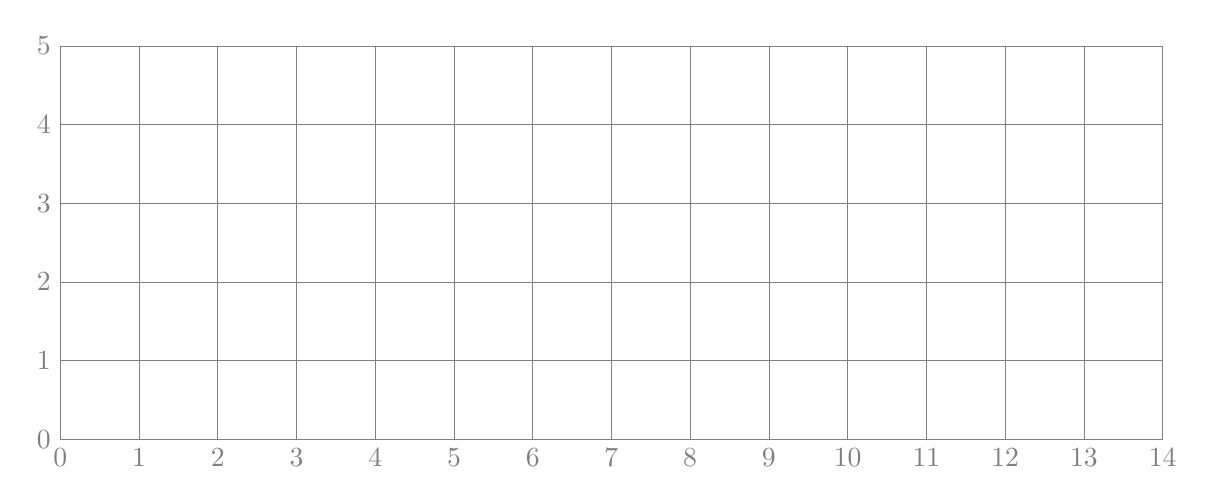
\begin{tikzpicture}
	 \foreach \i in {\xMin,...,\xMax} {
		\draw [very thin,gray] (\i,\yMin) -- (\i,5)  node [below] at (\i,\yMin) {$\i$};
	}
	\foreach \i in {\yMin,...,5
	} {
		\draw [very thin,gray] (\xMin,\i) -- (\xMax,\i) node [left] at (\xMin,\i) {$\i$};
	}
	
	%\draw [step=1.0,blue, very thick] (0.5,0.5) grid (1.5,1.5);
	%\draw [very thick, brown, step=1.0cm,xshift=-0.5cm, yshift=-0.5cm] (0.5,0.5) grid +(1.5,1.5);
	
\end{tikzpicture}
	\caption{The Git Pipeline: Working Tree, Staging Area and Commit Tree}
	\label{fig:GitPipe}
\end{figure}

 


\section{Commit, HEAD and local Branches}
\label{chapter:2.1}

This section is focused on summarizing briefly Git's meaning of commits, branches 
and referencing or addressing commits, respectively. We concentrate our investigations on the local 
.git repository. Concepts of fetch and merge, i.e. a pull operation and remote branching is part of \cref{chapter:3}. 



\subsection*{Commits}
  
Every commit represents a loaf in your commit tree. The whole commit tree represents the 
progress of your project. A single loaf or commit encapsulates 
your whole project at the time when the commit was made. That is, a commit is a snapshot 
of your project and you can extract that project state from just this single commit.
Each commit is unique and accessible through its identifying SHA-1 hash key.

The notion of commits is fundamental when using git. \textbf{Git is all about commits!} Especially the high level end user API of 
git is all about creating commits, pointing to or referencing special commits, grouping commits together,
looking inside a past commit, removing commits from your tree, restoring them etc.
But always remember, one single commit represents and contains your whole project at the time the commit 
was made.
   
Next to the commits, Git offers a set of pointers which are directed to special commits by default. These 
pointers are for addressing commits and investigating your commit tree. The set consist of:
\begin{itemize}
	\item HEAD pointer
	\item branch pointers
	\item origin/master pointer (refers to your remote commit tree)
	\item master or main branch pointer
\end{itemize}

Sections xxx and yyy concentrate on how to work with these pointers using the checkout and reset 
commands.


\subsection*{Local Git Branches}

The term branch often implies a somehow heavyweight and complex construct as part of the commit 
tree. In fact the contrary is the case. In the context of Git, a branch is nothing more then 
a named pointer directed on the latest commit in an directed, acyclic (sub-)graph of development
in the commit tree. That's it! Again, a branch is only a named pointer to a commit and the 
branch name represents a colletion of all commits with the same anchestor in the tree. However, although
we speak of pointers, these branch pointers are not meant to be moved freely around in your commit tree.
They are more like refereces and always refer to the latest commit in such an acyxlic graph.
In the following, the term branch means the whole acyclic (sub-)graph and the term branch pointer 
means the reference to the latest commit in this branch.
One special branch is the master or main branch.

\subsection*{Master/Main Branch}
The master or main branch reprents the trunk of your commit tree and is crated 
with the git init command. The master or main branch pointer is always directed to the latest commit added to 
this master branch. That is, creating a new commit also moves the pointer one commit further.

\subsection*{HEAD pointer, detached HEAD State}
The HEAD pointer is also created with the git init command. At the beginning this pointer is attached to 
the master pointer and refers to the same commit. Attached means, that the HEAD pointer is moved together 
with the master pointer. However, HEAD is designed as a real pointer and meant to be moved around in 
your commit tree. It is the git tool to reference arbitrary commits.
If the HEAD pointer (and only the HEAD pointer) is decoupled from the master pointer or any other branch pointer and moved backwards in time, i.e. to an older 
commit in the tree, one calls this state a detached HEAD.
To sum it up, the HEAD is directed to the commit which represents the the project state as you can see it, when you 
look in your current working tree.

\subsection*{origin/master} 
This pointer refers to the remote master branch inside the remote .git repository. Since this section only 
covers the local commit tree, the reader may consult chapter xxx for more information on remote HEAD and master
as well as remote branching. 
\\
Finally, figurexxx shows a picture of the commit tree in relation with the other trees and references
presented. It depicts the situation while adding a new commit and shows how new data gets assembled into a new commit.



\section{Git Reset}
\label{chapter:2.2}

\subsection{Three Types of Git Reset}
\label{chapter:2.2.1}

\subsection{Reset with Path Specification}
\label{chapter:2.2.2}

\section{Git Checkout, Switch and Restore}
\label{chapter:2.3}

\subsection{Detaching the HEAD}
\label{chapter:2.3.1}

\subsection{Git Restore}
\label{chapter:2.3.2}

Hello World!

%Finally, an example of how to add literature into the written text \cite{meyers2005effective}.

%It is also possible to specify pages with \cite[see][page 127]{arens2015mathematik}.